\documentclass[11pt]{article}
\input{\string~/.macros}
\usepackage[a4paper, total={7in, 9in}]{geometry}
\usepackage{bbm}
\usepackage{mathrsfs} % really cursive alphabets
\usepackage{graphicx}
    \graphicspath{{./assets}}
\usepackage{hyperref}
    \hypersetup{colorlinks=true, linktoc=all, linkcolor=blue, citecolor=red}
\usepackage[backend=bibtex,sorting=none]{biblatex}
\usepackage[margin=0cm]{caption}

% random variables
\newcommand\ry{\ensuremath{\mathsf{y}}}
\newcommand\rx{\ensuremath{\mathsf{x}}}
\newcommand\rb{\ensuremath{\mathsf{b}}} 
\newcommand\rc{\ensuremath{\mathsf{c}}}
\newcommand\rz{\ensuremath{\mathsf{z}}}
\newcommand\ru{\ensuremath{\mathsf{u}}}
\newcommand\rw{\ensuremath{\mathsf{w}}}
\newcommand\rpa{\ensuremath{\mathsf{pa}}}
\newcommand\rU{\ensuremath{\mathsf{U}}}
\newcommand\rbx{\ensuremath{\mathsf{\mathbf{x}}}}
\newcommand\rby{\ensuremath{\mathsf{\mathbf{y}}}}
\newcommand\rbu{\ensuremath{\mathsf{\mathbf{u}}}}

\newcommand\bbP{\ensuremath{\mathbbm{P}}}
\newcommand\bbQ{\ensuremath{\mathbbm{Q}}}


% boldsymbols
\renewcommand\bmu{\ensuremath{\boldsymbol{\mu}}}
\newcommand\bSigma{\ensuremath{\boldsymbol{\Sigma}}}
\newcommand\bgamma{\ensuremath{\boldsymbol{\gamma}}}
\newcommand\bomega{\ensuremath{\boldsymbol{\omega}}}
\newcommand\bnu{\ensuremath{\boldsymbol{\nu}}}


% optimization, classes of functions
\newcommand\scrF{\ensuremath{\mathscr{F}}}
\newcommand\scrS{\ensuremath{\mathscr{S}}}
\newcommand\scrP{\ensuremath{\mathscr{P}}}

% independence
\newcommand{\dperp}{\ensuremath{\perp\!\!\!\perp}}
\newcommand{\ndperp}{\ensuremath{\not\!\perp\!\!\!\perp}}

% operators
\newcommand{\prox}{\ensuremath{\mathsf{prox}}}
\addbibresource{kernel.bib}

\begin{document}
 
\section{Support Vector Machines}


Support vector machine is a kernelized optimal margin linear classifier (original paper \cite{boserTrainingAlgorithmOptimal1992} and a nice summary \cite{vertPrimerKernelMethods2004}). It distinguishes itself from classifiers minimizing empirical risk as it favors classifier which makes confident predictions. For binary classification problem $\sY=\pc{-1,+1}$, we are interested in finding a linear decision bondary, parameterized by $w\in\R^d,b\in\R$, that separates the training data points by maximizing the worst case distance (margin) of each data point to the decision boundary. We first assume that training set can be linearly separated. Given dataset $\pc{(x_i,y_i)}_{i=1}^n$, we are interested in solving the following quadratic programming problem,
\begin{align*}
    \min_{w,b}
        \;& \frac{1}{2} \norm{w}^2 \\
    \text{s.t.}
        \;& y_i(w^Tx_i + b) \geq 1 \quad i=1,2,\cdots,n
\end{align*}
To derive the dual problem, we write the Lagrangian, 
\begin{align*}
    \sL(w,b,\alpha)
        &= \frac{1}{2} \norm{w}^2 + \sum_{i=1}^n \alpha_i \pb{ 1 - y_i(w^Tx_i+b) }
\end{align*}
where $\alpha = \pc{\alpha_i}_{i=1}^n$ are the dual variables. Solve for $\inf_{w,b} \sL(w,b,\alpha)$ to arrive at the dual objective. In particular, first order optimality condition gives $w = \sum_{i=1}^n \alpha_i y_i x_i$ and it must be that $0=\sum_{i=1}^n \alpha_i y_i$. Therefore, 
\begin{align*}
    \max_{\alpha}
        \;& \sum_{i=1}^n \alpha_i - \frac{1}{2} \sum_{i=1}^n\sum_{j=1}^n \alpha_i \alpha_j y_i y_j x_i^Tx_j \\
    \text{s.t.}
        \;& \alpha_i \geq 0 \quad i=1,2,\cdots, n
            \tag{dual feasibility} \\
        & \sum_{i=1}^n \alpha_i y_i = 0 
            \tag{from $\nabla_b \sL = 0$}
\end{align*}
The dual can be solved more efficiently than the primal problem using coordinate descent. The decision rule is linear w.r.t support vectors (those $x_i$ right on margin with $\alpha_i > 0$)
\begin{align*}
    \hat{y}(x) = \text{sgn}\left(
        \sum_{i=1}^n \alpha_i y_i x_i^T x + b
    \right)
    \quad\text{for}\quad
    b 
        = y_i - \sum_{j=1}^n \alpha_j y_j x_j^T x_i
\end{align*}
for any support vector $x_i$. We observe that optimization as well as prediction uses input vectors via dot products only. We are motivated to use feature mapping $\phi:\sX\to\sH$ to map input vectors to a higher dimensional possibly infinite feature space in hope that the lifted space is linearly separable. The kernel function $k: \R^d\times\R^d \to \R$ allows us to compute dot products $k(x_i,x_j)=\inner{\phi(x_i)}{\phi(x_j)}_{\sH}$ efficiently and represents a notion of similarity over two instance of aribtrary objects, e.g. vectors in $\R^n$, graphs, texts. We can substitute $k$ whenever inner product is used and arrive at a optimal margin classifier over implicitly defined nonlinear feature mapping $\phi$. In case when training dataset is not linearly separable, we can introduce slack variable $\pc{\xi_i}_{i=1}^n$ where $x_i\geq 0$ to relax the inequality constraints and penalize misclassified or within margin points with $C\sum_{i=1}^n \xi_i$ for some $C\in\R$. In this case, we have the following Lagrangian,
\begin{align*}
    \sL(w,\xi,\alpha,\beta)
        = \frac{1}{2}\norm{w}^2 + C\sum_{i=1}^n \xi_i + \sum_{i=1}^n \alpha \left( 1-y_i ( \inner{w}{\phi(x_i)}_{\sH} + b )-\xi_i \right) + \sum_{i=1}^n \beta_i \xi_i
\end{align*}
First order condition $0 = \frac{\partial}{\partial \xi_i}\sL = C - \alpha_i + \beta_i$ together with dual feasibility $\beta_i\geq 0$ yield $\alpha_i \leq C$ for all $i=1,2,\cdots,n$. Therefore, we optimize for the following dual problem,
\begin{align*}
    \min_{\alpha}
        \;& \frac{1}{2} \alpha^T Q \alpha - 1^T \alpha  \\
    \text{s.t.}
    \;& y^T\alpha = 0 \\
    \;& 0\leq \alpha_i \leq C \quad i=1,2,\cdots, n
\end{align*}
where $Q \in \R^{n\times n}$ with $Q_{ij} = \alpha_i \alpha_j k(x_i,x_j)$,
with optimal decision rule as
\begin{align*}
    \hat{y}(x) = \text{sgn}\left(
        \sum_{i=1}^n \alpha_i y_i k(x_i,x) + b
    \right)
    \quad\text{for}\quad
    b = y_i - \sum_{j=1}^n \alpha_j y_j k(x_j,x_i)
\end{align*}
for any support vector $i$, i.e. $0 < \alpha_i < C$.

\begin{center}
\begin{figure}[h!]
    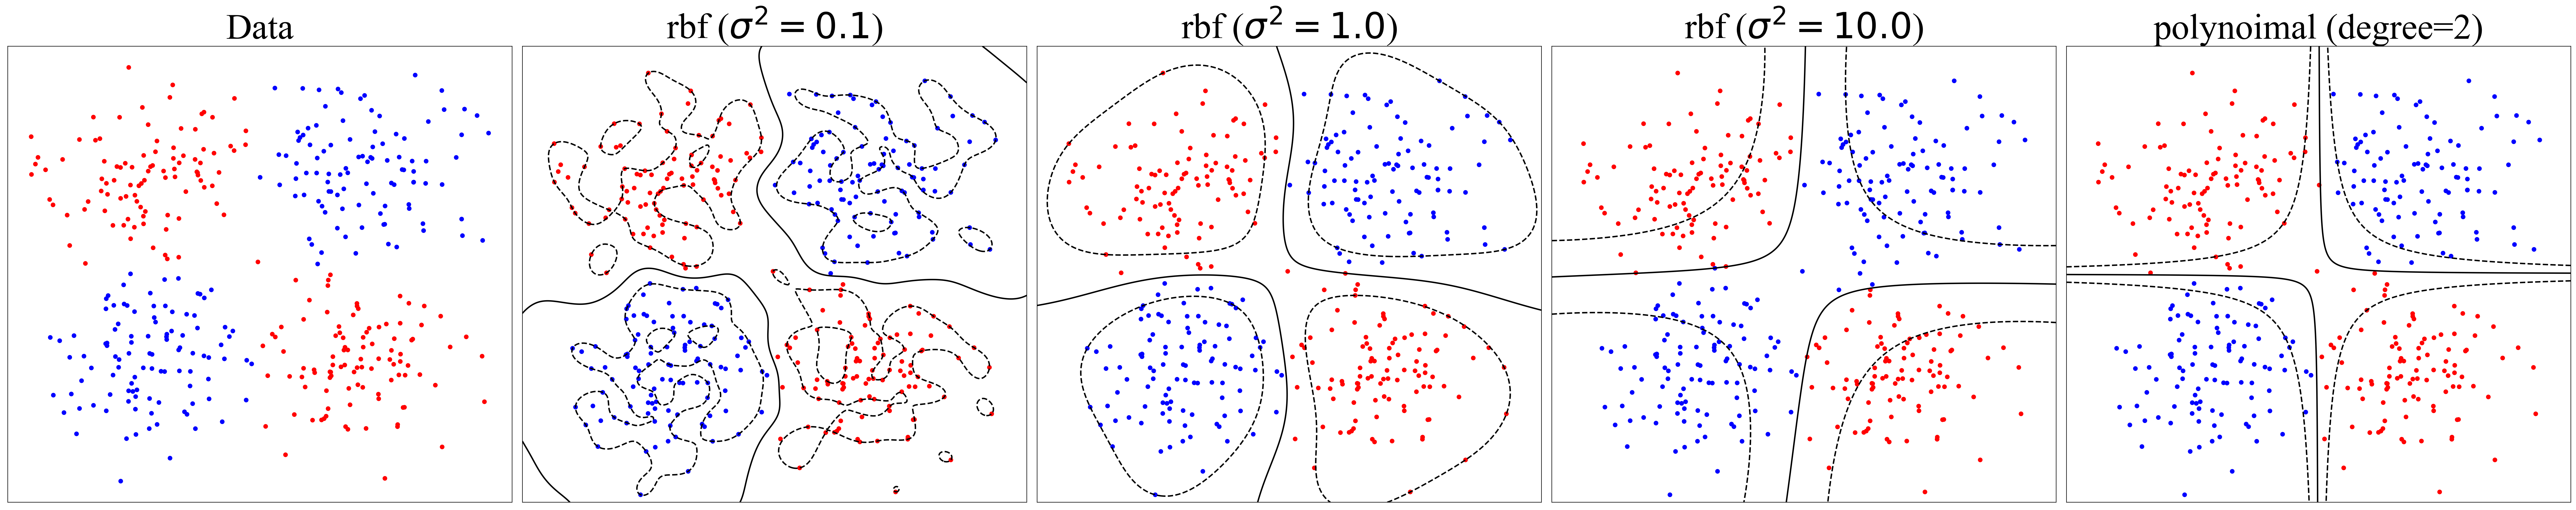
\includegraphics[width=\textwidth]{assets/svm_on_2d_gaussian_vary_kernel.png} 
    \caption{SVM on simulated 2D Gaussian with degree two polynomial kernel and radial basis function kernel with varying bandwidth. Larger bandwidth corresponds to smoother decision boundary and in the limit approaches the decision boundary of a linear kernel}
\end{figure}
\end{center}


\section{Reproducing Kernel Hilbert Space}

\cite{grettonWhatRKHS2012} provides a rigorous introduction to RKHS while \cite{grettonIntroductionRKHSSimple2019} provides pretty good intuitions. 

\begin{definition}
    (Hilbert space) A Hilbert space is a complete inner product space, i.e. $(\sH, \inner{\cdot}{\cdot}_{\sH})$
\end{definition}

\begin{definition}
    (Reproducing kernel Hilbert space) A Hilbert space $\sH$ of functions $f:\sX\to\R$ is a RKHS if its evaluation functional, $\delta_x:\sH\to\R$ where $\delta_x(f) = f(x)$ is continuous $\forall x\in\sX$.
\end{definition}

Intuitively, RKHS is a space of well-behaved functions. In particular, norm convergence in $\sH$ yield pointwise convergence, i.e. $\lim_{n\to\infty}\norm{f_n-f} = 0$ implies $f_n \to f$. Note evaluation functional is linear. The condition that $\delta_x$ is continuous is equivalent to $\delta_x$ be bounded \cite{grettonWhatRKHS2012}.

\begin{definition}
    (Reproducing kernel) Let $\sH$ be Hilbert space defined on non-empty $\sX$, then a function $k:\sX\times\sX\to\R$ is called a reproducing kernel of $\sH$ if
    \begin{enumerate}
        \item $\forall x\in\sX$, $k(\cdot,x)\in\sH$ 
        \item $\forall x\in\sX$, $\forall f\in\sH$, $f(x) = \inner{f}{k(\cdot, x)}_{\sH}$ (reproducing property)
    \end{enumerate}
    In particular, for any $x,y\in\sX$, $k(x,y) = \inner{k(\cdot,x)}{k(\cdot,y)}_{\sH}$.
\end{definition}

Note the reproducing kernel $k$ can be represented as an inner product of image over $\phi:x\to k(\cdot,x)$, i.e. $k(x,y) = \inner{\phi(x)}{\phi(y)}_{\sH}$ . It turns out that RKHS has $\sH$ is a RKHS if and only if $\sH$ has a reproducing kernel. Definition of RKHS based on continuous evaluation functional is equivalent to existence of a (unique) reproducing kernel. 

\begin{definition}
    (Positive definite functions) A symmetric function $h:\sX\times\sX\to\R$ is positive definite if for all $n\geq 1$ and for all $(a_1,\cdots,a_n)\in\R^n$ for all $(x_1,\cdots,x_n)\in\sX^n$, 
    \begin{align}
        \sum_{i=1}^n \sum_{j=1}^n a_i a_j h(x_i,x_j) \geq 0
    \end{align}
\end{definition}
If you consider a function $k:\sX\times\sX\to\R$, $k$ is positive definite if any kernel matrix $K\in\R^{n\times n}$ where $K_{ij}=k(x_i,x_j)$ is positive definite, i.e. $K\succeq 0$. 

\begin{definition}
    (Kernel defined via feature map) Let $\sX$ be non-empty set. The function $k:\sX\times\sX\to\R$ is a kernel if there exists a real Hilbert space $\sH$ and a map $\phi:\sX\to\sH$ such that $\forall x,y\in\sX$, $k(x,y)=\inner{\phi(x)}{\phi(y)}_{\sH}$. $\phi$ is said to be the feature map and $\sH$  be the feature space.
\end{definition}

Note there maybe more than one feature map yield for any one kernel. Intuitively, a kernel is a function that can be represented as inner product. It turns out that RKHS with reproducing kernel $k$ is positive definite,
\begin{align}
    \sum_{i=1}^n \sum_{j=1}^n a_i a_j k(x_i,x_j)
        = \sum_{i=1}^n \sum_{j=1}^n a_i a_j \inner{k(\cdot,x_i)}{k(\cdot,x_j)}
        = \inner{\sum_{i=1}^n a_i \phi(x_i)}{\sum_{i=1}^n a_i \phi(x_i)}_{\sH}
        \geq 0
\end{align}
and, conversely, we can show that for every positive definite function $k$ there corresponds to an unqiue RKHS whose reproducing kernel is $k$ (Moore-Aronsajn). Intuitively, we construct a RKHS $\sH = \overline{\sH_0}$, the completion of a pre-RKHS space $\sH_0 = \text{span}(\pc{k(\cdot,x)}_{x\in\sX})$. In particular, the choice of inner product 
\begin{align}
    \inner{f}{g}_{\sH_0}
        = \sum_{i=1}^n\sum_{j=1}^m \alpha_i \beta_j k(x_i,y_j)
\end{align}
for $f = \sum_i \alpha_i k(\cdot,x_i), g = \sum_j \beta_j k(\cdot, y_j)$ makes $\sH_0$ a valid pre-RKHS. Intuitively, this construction implies that RKHS is a space spanned by $\pc{k(\cdot,x)}_{x\in\sX}$ or by feature maps $\pc{\phi(x)}_{x\in\sX}$.



\newpage
\printbibliography 




\end{document}